\documentclass[a4paper, 10pt]{article}

\usepackage{graphicx} %%Good primer on this see:  https://www.youtube.com/watch?v=Ax9RCvjpI8E

\usepackage{geometry} %%To set basic page parameters. See also: https://www.overleaf.com/learn/latex/Page_size_and_margins
\geometry{a4paper, portrait, margin=1in}

%%Use this when you want to change colors eventually: https://tex.stackexchange.com/questions/75667/change-colour-on-chapter-section-headings-lyx

%%This is a function I found on stack overflow when I looked up
%%'How can I change the margins for only part of the text?'
\def\changemargin#1#2{\list{}{\rightmargin#2\leftmargin#1}\item[]} 
\let\endchangemargin=\endlist 
%%Use it sparingly.

\renewcommand \thesection {\Alph{section}} %%Defines section numberings (A.1.1, etc)

\begin{document}

\begin{titlepage}

	\begin{figure}[h]
		\centering
		
\includegraphics[scale=.8]{HackRoverlogolofi}
	\end{figure}

	\begin{center}
		\vspace*{1cm}
	
		\Huge
		\textbf{HackRover}\\[10pt]
	
	
		\large
		\textbf{Capstone MegaDoc}\\[40pt]

		\begin{changemargin}{10pt}{10pt} 
		\begin{center}
		\normalsize
		Justin Heinzig, Danny Kha, Jacob Park
	
		Advisor; Mentor; Sponsor: Pierre Mourad\\[150pt]
		\end{center}
		\end{changemargin}
	\end{center}
	
	\begin{figure}[h]
		\centering
		
\includegraphics[scale=.8]{UWLogo}
	\end{figure}		
	
\end{titlepage}

\pagebreak{}

\tableofcontents

\pagebreak{}

\section*{Foreward}
	\subsection*{Abstract}
	----This is a meta section about how this paper is ordered.	
	
	\subsection*{Executive Summary}
	HackRover is a cyber-defense-based student research project aimed at making, breaking, and hacking mobile platforms, encompassing rovers, drones, and anything that moves. Our goal is to practice and develop skills to help defend our increasingly connected world of embedded systems, where the safety of people and communities is being placed in the hands of autonomous machines.
	
	Our plan is to pioneer a new type of hacking competition - named the HackRovoer Autonomous Robotics Competition (HARC) - where participants attempt to infiltrate self-driving rovers and collect round-winning information. There is no hackathon in the world that is centered around autonomous machines, yet according to a 2019 Global Autonomous Driving Industry Outlook report, 1 in 4 cars are expected to have autonomous capabilities by 2030. The competition we’re creating isn’t exclusive to UW Bothell, as tentatively schools around the globe can set up chapters. Succeeding in creating such an event would result in an excellent pedegogical tool. 
	
	Each iteration of the competition the theme changes, which influences competing rovers' designs, puzzles and props within the competition, and game rules. This iteration's theme is disaster relief; participants are tasked with designing rovers which find themselves in disasters like collapsed buildings or tornado paths. They'll build rovers for a hypothetical company which would sell to local governments and emergency services in disaster prone-regions. Rovers would provide mostly scouting and minimal medical function, either/both seeking out victims (such as under rubble) or/and dispensing minimal medical aid. Obviously the competition is yet to exist officially, so we act as a lone team following the themes set for ourselves. 
	
	This year we completed the construction of a disaster rover (first iteration), nicknamed Mimir, as well the competition puzzle panel, a prop which the rover interacts with. The rover we designed consists of three tiers stacked onto a drive base: the bottom tier houses microcontrollers and electronic power distribution; the middle tier houses the microcomputer and communication devices; and the top tier houses the LiDAR camera system and its control Stewart platform. The puzzle panel contains small electromechanical devices mounted by velcro to a velcro-clad, wooden puzzle; these devices are currrently interfaced by an Arduino Mega and custom design, PCB power distribution system (PDS). See below are the two devices completed this quarter.

	--------------------ADD THE IMAGES
	
	------------------------------------------
	
\pagebreak

	\subsection*{Project Requirement Documentation}
	The disaster rover we're building must be debris resistant and capable of traversing non uniform terrain. Functionally it must be controllable over a wireless connection (network satellite or otherwise) with a standard XBox gaming controller or keyboard. It should send any and all sensor data back through the connection to a browser-based GUI; this quarter the data will at minimum include LiDAR camera images. Internally the rover needs: (1) a PDS to provide 12V and 5V through various means, (2) a central command microcomputer capable of making all necessary high level logical decisions, (3) microcontrollers capable of communicating control commands to the rover drive train and LiDAR's position control device, and (4) networking devices enabling the rover to be operated wirelessly. The PDS should provide clean energy to motors and logical devices simultaneously, as well as present additional 'ports' for future devices and add-ons. The central command microcomputer should be capable of interfacing with all control components, operating at a high level (with the GUI and user), and centralizing control. The microcontrollers should forward information to the control mechanisms (servos, motor controllers, etc) from the central microcomputer. The networking devices must provide switch functionality, to interconnect devices within the rover, routing functionnality, to interface the rover with outside networking, and wireless access.
	
	The puzzle panels for the competition should emphasize easy engineering: mechanical, electrical, and computer. Mechanically, devices should be easily and reliably mounted and interfaced on a flat board. Options for configuration should be provided for maximum puzzle design creativity. Electrically, all components should have access to clean power through a simple panel PDS without significantly effecting the power recieved by other components. Signals must be sent into and out from an Arduino central microcontroller with ease. Computer-wise, components should have code libraries created for easily prototyping and producing a myriad of puzzle arrangements. Students unfamiliar with programming should be able to learn and create with short lead time, and not have to worry about seeking out libraries or software components for themselves. 
	
\pagebreak

\section{Design Strategy}
	\subsection{User Insights and Research} 
		\subsubsection{Consumer Journey Map}
		The unique nature of our project makes consumer analysis difficult, as product consumption occurs at multiple levels: faculty, students, companies, disaster responders, etc. Here we'll speak lightly of most and provide consumer journey maps for students and disaster responders: the key subjects of our capstone project.
		
		When structuring education, university faculty seek useful pedegogical tools; such tools will provide  interdisciplinary education, equip students with life skills, and possibly generate research/products that enrich the name and wealth of the school. Students, specifically engineering ones, look to develop their skills while in school through participation in clubs, projects, and research. They're often pulled in many directions as their educational appetite is wide but options are slim/focused.
		
		-----NEED IMAGE OF STUDENT CONSUMER MAP: The student should look for extracurriculars, see options, have to pick an option, each option should have different benefits. Something like that.
		
		Seen above is a student consumer map cataloguing the journey a student experiences as they seek extracurricular, educational activities which empower them. A key takeaway is that the student is limited by time and must select one club with a narrow purpose. Further, these clubs demand a wealth of previous knowledge and experience to properly participate, raising the bar to entry. Broadening the scope of work for any given organization and lowering the bar to entry are obvious improvements.
		
		Robotic companies that develop disaster rovers are limited by the opportunities available to them and niche of their field. Disaster relief is a philanthropic endeavour for the most part, where the only money to  be made is from tech savvy local governments (an already fickle customer) or when disaster relief can be repurposed as a virtuous advertisement. Minimal money exists in prize form through government sponsored competitions or events, like DARPA's disaster relief competition. Beyond monetary opportunity, research is hard to come by; like an ouroboros, the lack of monetary gain causes people to ignore robotics research in disaster relief. This makes constructing disaster relief systems difficult all around. A disaster responder's role all of this makes R\& D even more difficult, as relying on robotic systems is a difficult and risky endeavour. You're never sure when a disaster will strike, and circumstances are unique each time. As a responder you must delegate quickly and make use of limited resources in saving as many lives and limiting damage as possible. Rovers are dependent on a human operator as well as some uptime; further, their operation needs to be clean and quick to permit a disaster responder to complete the same or better task without major risks.
		
		------NEED IMAGE OF STUDENT CONSUMER MAP: The disaster responder should be presented with a disaster, have to quickly assess damages, delegate  resources in a timely manner, save people, make risks. Possibly emphasize the risks they might take, and talk about the time it takes to accomplish their goal. 
		
		Seen above is a disaster responder consumer map cataloguing their response to a generic disaster event. Of emphasis is the risk to responder's life, a time crunch, and quick decision making with limited resources and information. Systems or methods that might remove the human operator from danger, improve operation efficiency, and maximize life-saving information and resource use are obvious improvements.
		
		
		\subsubsection{Stakeholder Framing}		
			\begin{itemize}
			\item
			\textbf{Stakeholder:} \emph{Government Relief Organizers:} The bottom line of these individuals is effective distribution of force and resources; inability to do this casts doubt on their ability. Any cost effective solution which improves how they distribute resources, or reduces resources needed will be a boon to them. 		
			
			\item
			\textbf{Stakeholder:} \emph{Disaster Relief Operators:} Like the government organizers above, these individuals need to manage a swath of resources; albeit smaller, with more attention. Tools that can sub in for more expensive resources, have shorter uptimes, improve information gathering, accomplish rescue, and maximize human life (operator or victim) are beneficial.
			
			\item
			\textbf{Stakeholder:} \emph{UW Bothell Students:} UW Students are the primary beneficiaries of our product. Prior we made clear the intent to create a product that serves UW Bothell students first and foremost, and whose reprocussive effects are benefits to disaster response. Providing students with extracurricular engineering activities that are easy to get into while simultaneously serving broad interests will nix the problem of narrow-focus clubs with steep learning curves. 
			
			\item
			\textbf{Stakeholder:} \emph{UW Capstone Core Team:} Our organization already exists, but the product we create will have bearing on our success. The ability to serve a  need within the school has direct correlates to further funding and participation.

			\item
			\textbf{Stakeholder:} \emph{Pierre Mourad:} Pierre derives benefits from the product in the form of reputation of his person, outreach for access to students (for other projects potentially), and access to robotics systems. Our performance in this capstone cycle will affect trust in his decisions.
			
			\item
			\textbf{Stakeholder:} \emph{UW Faculty:} Like Pierre, the UW faculty has a stake in this project. They've provided plenty of resources and space which might be used for something else. Further, a successful project might provide a powerful pedagogical tool in the future.

			\item
			\textbf{Stakeholder:} \emph{UW Student Technology Fund:} The STF is the primary contributor to our organization, providing more than 3000 dollars in hardware technology. The exchange of this technology was meaningful use, future requests need to be paired with demonstration of this good use.
			\end{itemize}
			
			
		\subsubsection{User Scenarios and Personas}
		\subsubsection*{Three Personas:}
		\begin{itemize}
			\item
			
			\emph{UW Student seeking a club} A prototypical UW engineering student seeking out extracurriculars to further their knowledge of mechanical, electrical, and/or computer  engineering. 
			
			\item
			\emph{UW Faculty seeking new educational resource} A UW faculty member desiring to contribute to the education of their students while generating value within the school.
			
			\item
			\emph{Disaster responder} A diasaster responder on the ground attempting to respond to an earthquake that resulted in the collapse of multiple buildings with people inside.
		\end{itemize}
		
		
		\subsubsection*{Scenarios:}
		\begin{itemize}
			\item
			A students looks at a roster of available clubs and organizations to participate in with the aim of furthering their engineering ability in multiple fields and equipping them with industry-standard skills. They're met with a limited selection containing clubs that exist but don't operate well, and others which are popular; all of these clubs have a niche focus that forces the student to sacrifice some of their interests if they invest their time. The student picks a popular club and is met with a great amount of competition and steep learning curve. Everyone wants to contribute and do something cool, but resources are limited, so competition ensues. To stand out the student  must struggle to learn a massive amount of content; by the end their skills may no longer  be useful. Trying to latch onto existing projects within the club is difficult because documentation is sparse and the student can't understand decisions that were made. These circumstances aren't different for others so the project sits in gridlock: afraid to move forward in case precious resources are destroyed during the process of improvement, and a lack of confidence in how to move forward, since decisions require immennse background knowledge (which isn't well documented). The student spends most of their time jumping hurdles just to do minimal meaningful engineering, get discouraged, and use the club as a resume filler.

			\item
			A faculty member has to balance their desire to improve their students lives with forwarding their own career. They could create a product which is a horrible pedagogical tool and hyper-focuses the education of their student, but which benefits their own reputation and school image. Alternatively they create product which is great for educating students, but doesn't draw any attention or produce meaningful results/research. 
			
			\item
			A disaster responder is provided a small troop of men to command with limited expensive resources to save as many lives as possible in a short amount of time. If they spend too much time deliberating, hundreds may be crushed or suffocated under rubble; if they act too quickly manpower and resources will be spent inefficiently, hundreds may still die. Information collection and action must also be balanced. Any work they do also places their own team-members lives' at risk.
		\end{itemize}
		
		\subsubsection*{One Scenario Environment}
		The environment of focus is the disaster responder since it's scenario which motivates most development decisions within the project. The student is important but accessory to the disaster responder. We've repeatedly emphasized above the time and resource intensive environment responders participate in, increased consideration to human life, and limited information. Furthermore, disaster responders are beholden to government organizers who provide resources for disaster response. Despite being the users of our product, the responders must be able to convince higher ups the acquisition is sensible and cost-effective.

		\subsubsection{User Insight Report}
		\textbf{UW students} need a product that address their lack of interdisciplinary, extracurricullar activities. acitivities provided by the product must be friendly to students of any educational background and not require them to climb a steep learning curve; documentation of past activities should be plenty yet easy to read. Clerical work should be minimized, while real engineering work is maximized. Any participation should result in industry skills being learned.
		
		\textbf{UW faculty} members need a product that is both pedagogically developed and useful for producing reputable work and/or research. 		
		
		A given of our capstone is the development of some rover that addresses disaster responders' issues, beyond additional product components which address UW students' needs. We've made it very clear that \textbf{disaster responders} need a rover design that's cost effective, as to convince government organizers of acquisition; has a short up-time and is easy to control, to maximize efficiency; and, can provide vital information, to streamline rescue missions and better distribute resources.
		
		A few meetings with our sponsor, Prof. Pierre Mourad, shed light on both the school environment and state of disaster relief robotics. It seems Bothell suffers from limited engineering extracurriculars, many of which are too narrow (as per our previous mention); the only solid `rover' project is TrickFire, which sees heavy member competition. Furthermore, few pedagogical tools exist for students; many try to learn through clubs, but those often require extensive background understanding. Pierre Mourad  also discussed his understanding of disaster relief rover design: companies would rather send a specifically configured rover into the situation substitute for a responder, but close by. Rovers would need to be easily configurable or provide enough data under small up-time to legitimize their use in the field. Rovers should also have some autonomous  function so they don't have to be babysat by their operators.

	\subsection{Problem Understanding}
		\subsubsection{Product Assumptions}
			\begin{itemize}
			\item
			For UW Students: A product that addresses their lack of interdisciplinary, beginner-friendly extracurriculars, which improves their education, equips them with industry-standard skills, and provides an outlet for creative design. 
				
			\item
			For UW Faculty: A product that addresses their lack of pedagogical tools \& reputable student projects, providing benefit in the form of an excellent learning tool they might direct students towards while simultaneously generating projects that advance the school's reputation.
		
			\item		
			For disaster responders: A product that addresses their time \& resource constraints while responding to disasters, and concern for human life, by providing life-saving information (or even saving lives) with little up time, small cost to direct supervisors, and ease-of-use. 
			\end{itemize}


		\subsubsection{Functional Assumptions}
			\begin{itemize}
			\item 
			For UW Students: A product that addresses their lack of interdisciplinary, beginner-friendly extracurriculars, which improves their education, equips them with industry-standard skills, and provides an outlet for creative design, via that product's pedagogical methods, emphasis on industry practice, and interesting activities. 
		
			\item		
			For UW Faculty: A product that addresses their lack of pedagogical tools \& reputable student projects, providing benefit in the form of an excellent learning tool they might direct students towards while simultaneously generating projects that advance the school's reputation, via that product's pedagogical methods, and activities that generate documentation and design research. 
		
			\item
			For disaster responders: A product that addresses their time \& resource constraints while responding to disasters, and concern for human life, by providing life-saving information (or even saving lives) with little up time, small cost to direct supervisors, and ease-of-use, via that product's data collection systems, simple configuration, cheap yet robust construction, and intuitive controls.	
			\end{itemize}
		

		\subsubsection{High Level Usability Constraints}
			\begin{itemize}
			\item 
			For UW Students: An accessible, well funded, educational product that addresses their lack of interdisciplinary, beginner-friendly extracurriculars, which improves their education, equips them with industry-standard skills, and provides an outlet for creative design, via that product's pedagogical methods, emphasis on industry practice, and interesting activities. 
		
			\item		
			For UW Faculty: A well-documented, effectively managed, economically efficient educational product that addresses their lack of pedagogical tools \& reputable student projects, providing benefit in the form of an excellent learning tool they might direct students towards while simultaneously generating projects that advance the school's reputation, via that product's pedagogical methods, and activities that generate documentation and design research. 
		
			\item
			For disaster responders: A short up-time, easy-to-use product that addresses their time \& resource constraints while responding to disasters, and concern for human life, by providing life-saving information (or even saving lives), and small cost to direct supervisors, via that product's data collection systems, simple configuration, cheap yet robust construction, and intuitive controls.	
			\end{itemize}

		\subsubsection{Final Need Statement and User Outcomes}
		\textit{A short up-time, easy-to-use product which considers the time \& resource constraints of disaster responders while providing life-saving information. The product will certainly be a rover, easy to configure and operate, cheap, and with robust data collection systems, altogether easy to control. The entire rover will be developed within the context of an undergraduate robotics competition, where competition props (mostly electromechanical) and guidelines will serve as pedagogical tools, and all student activities will be documented according to industry standards, (documentation technology and formats).}
	
		This is a tricky two-part needs statement: (1) the rover portion of the product for the disaster responders, and (2) the product satisfying the needs of the students. The aim was to direct student efforts and learning to the construction of the physical product; this directed effort is accomplished through the pedagogical tool which is the competition. 

		\subsubsection{Hypothesis Statement}
		For the disaster responders, the product is obviously going to be a rover. For simplicity of prototyping we're going to design a earthquake disaster response rover. We believe a system which is dust and rubble resistant, capable of semi-autonomous action, collecting and relaying data, cheap to manufacture, and easy/quick to setup will help in information collection and decision making for disaster response teams, and potentially serve functions traditionally held by human responders, preserving human life. 
		
		This physical product will be prototyped within some educational setting which acts as the abstract, student-serving component of the product. We're the educational setting is going to be a competition, but the specifics of the guidelines are unclear as of now. The competition would be managed by our organization, which is both a club and capstone. 

		\subsubsection{Possible Inventions and Business Model}
		-----Needs a discussion of:
		1. A bunch of different inventions that exist today and their shortcomings
		2. Inventions WE might create; emphasize us creating inventions that only satisfy part of the problem, like a rover body with minimal sensors, then a sensor stack, etc. Or, different 'versions' of the competition which don't actually exist. Use flow chart tools to visualize the inventions. 
			
		Further discussion with Mourad generated ideas for the informed us that we might pivot HackRover to design competitions which reward designs suiting disaster situations by creating simple puzzle elements and point systems which reward the related functions. The puzzles themselves act as a springboard for our design direction. Further, multiple rovers of various configurations will be built simultaneously to see ‘what works’. This will provide first responders with an arsenal of quickly configurable rovers that can be used in any type of disaster scenario, or at least lead to the design of one ‘great’ system spread nebulously in the design of all four systems.		
		
		\subsubsection*{Possible Inventions:}
		Current systems for disaster relief are overly-expensive, shallow attempts at a design that jerry-rig existing structures/systems to solve issues of disaster relief. What’s more is that these systems rarely provide meaningful help, have large uptimes, or return limited data back. For example, aerial systems show snapshots from a bird's eye view, but little more; they're expensive to acquire, time-consuming to deploy, and require a skilled operator. Some might argue that visual feedback is enough to trace access paths and gauge the scope of the damage, but it gives a limited understanding of victim locations, danger points, etc. Another example: most land rovers - despite being capable in their locomotion - return limited useful sensor data (compared to drones), and the current state of actuative technology is limited. The biggest thwart to effective disaster technology, however, is the context in which it's developed. Frequently made by heavy industry tech giants, the return on investment is minimal and opportunity costs are great; to them, the effort is best served elsewhere. The only place to turn to, then, is University Students who are willing and wanting to work for the low cost of a good resume and contribution to society. Here effective organizations need to be made to mobilize their talents into the creation of disaster relief robots; the best scenario is a robotics competition. Most existing competitions see students participating in events that see them designing rovers tailored to useless/limiting activities, or just working with a confining kit and no creative freedom at all. Though some break the mold, they're few and far in between, and none focus on disaster relief. To further robotic, disaster relief tech, effective student organizations must be created.
		
	The first obvious 'invention' of this capstone is a disaster relief-oriented competition, which we call the HackRover Autonomous Robotics Competition (HARC). Traditionally it existed to provide an outlet for interdisciplinary engineering practice and an exploration of IoT; but, as the competition itself has no context there is a point for improvement. This new iteration emphasizes the creation of puzzle panels with elements and a point system that inspires the design of autonomous systems with capable actuation, computer vision and vision processing, capable locomotion, short up-time, easy configuration, and quick access.

The second main invention is a modular rover framework. In the past, the biggest hurdle for all robotic systems has been the software architecture, which must be uniquely tailored to the hardware being employed. With the help of some middleware Robotic Operating System (ROS), we can create individual software nodes and elements which can be knit together in as little as a day to create unique robotic software stacks. Our goal, then, is to create an easily understandable, well-documented, modular rover framework that supports a near-endless number of arms, locomotive systems (traditional mostly), cameras, and other sensors, limited only by the hardware being used.	

The third invention is a physical disaster relief rover. Founded on the modular rover software framework (discussed as invention two), the design of the relief rover would only concern a small group of electrical and mechanical engineers configuring various pieces of third-party hardware into a physical rover capable of speedy, robust locomotion, payload delivery, actuation, and sensing. All control (arm and locomotion), sensor data processing, and additional actuative capabilities are the subject of the well-designed software framework mentioned.

		\subsubsection*{Our Solution and Invention}
		\textit{An intuitively controlled disaster relief rover which considers the time \& resource constraints of disaster responders - with its short up time and inexpensive construction - while providing life-saving information from its sensor stack and various feedback mechanisms. The rover will be developed within an undergraduate robotics competition, where competition props (electromechanical) and guidelines will serve as pedagogical tools, and all student activities are documented in \LaTeX\ and akin to IEEE standards.}		
		
		Choosing to develop the rover within a competition setting both satisfies the needs of a pedagogical tool for UW Bothell students and produces the desired rover. The competition, we're calling the HackRover Autonomous Robotics Competition (HARC) will be held at Bothell, managed by the HackRover club and capstone project. The annual nature of the comeptition will serve as a force for iteration, making the design better year over year. The addition of hacking serves to penetration test rovers so they can't be taken advantage of while performing life-saving tasks. In a good-faith effort to bring the competition to life we will also be making puzzle-panels, which are competition props that the robotic systems interact with. These puzzle-panels are themselves pedagogical tools designed to teach students the basics of mechatronics design. Below is a representational image of the competition venue Discovery Hall for context. Puzzle elements are laid out on about four floors, accessible by stairs/elevators. Students operate rovers, attempting to solve puzzles and gain points while navigating the building effectively and hacking/slowing other competitors' rovers. Points are awarded based on solutions to puzzles, specifically designed to encourage rover designs that would be capable in disaster relief contexts.
		
		----------NEED  AN IMAGE HERE -----------
	
		Despite shortcomings early designs, the rover will serve as disaster relief in limited contexts and will provide an enriching educational engineering experience for UWB students now and for the future. The practice of documenting in \LaTeX\ will not only provide students with industry-standard skills, and aid at generating a wealth of information which might be used by other developers; but, it will also speak to the high standards of practice, and aide in on-boarding students with ease, lowering the learning curve.
	
		\subsubsection{Planning Roadmap}
		----Needs to be a planning roadmap of the build of the robot itself, not the actual project.
		\textbf{Initial Product:} A competition with a rulebook, at least two rovers (one disaster-relief oriented), and four puzzle panels.
		
		The first competition encourages student involvement, a clear understanding of the framework, and expectations for the iterative methods used in developing our systems. Puzzles won't be so disaster-tailored as much as they will be a proof of concept. The first two rovers created will be designed to prototype a 'skeleton' software framework that exemplifies the principles of the software organization we desire. Physically these rovers will serve different purposes: the first to simply prototype the competition, drive around Discovery Hall, and make use of our available technology, and the second to provide an early model of what a disaster relief rover could be. Focusing more on the latter robotic design, an early disaster relief rover would have quick, rugged locomotion systems, effective sensor data storage, feedback, and/or processing, capable payload delivery, and meaningful arm actuation. At this point in the 'product' development, we wouldn't focus too hard on waterproofing or extremely robust chassis. The obvious adopters here are going to be UWB students, capstone students, Pierre Mourad, STF, and only philanthropic companies.
		
		\textbf{Product Additions:} \emph{An improved, R and D-friendly, competition.}

	The competition will eventually be formatted to address the desires of tech companies nationwide. Interested investors can trade capital for limited control over the direction of the competition and design requirements of involved rovers. As the competition and participants grow this offer would be more lucrative, and the potential for outsourcing cheap but quality R\& D increased greatly.

		\textbf{Product Additions:} \emph{Specialized Software Nodes.}
		
	Mentioned implicitly through the document is the notion that software nodes 'providing/extending capability' of the rover may be created. A feature of ROS is that functionality can be compartmentalized to a web-like software architecture. Drastic changes in the hardware do not require extensive recreation of the software; instead, nodes are repurposed and reorganized to achieve a framework that reflects the physical system. A skilled ROS operator with knowledge of the nodes' functions could create a completely new system within a day, for a totally unique rover. Future product additions could see 'stacks' of nodes created for unique disaster relief settings: building collapse, fire, aqueous, etc. Each of these stacks would come with the necessary code to configure context-specific locomotion, sensing, and actuative systems. Instead of purchasing an expensive system that 'does it all', clients could buy just one software stack suited to their disaster response expectations. 
	The rovers' modularity will have different packages that a client can use to configure their rover to their specification. For example, if there is a need for a LIDAR system then there is a module that would integrate the LIDAR system for a client. This would already be done physically as a unit that would attach with one connector to the main rover board and the software would just have to have slight code changes to adapt to the new module. 

\pagebreak
	




\section{Experience Design and Human Interface Design}
	\subsection{User Workflow}
	------Needs to discuss how someone might use the rover and devices. Talk about within the competition and how it interfaces with the puzzle panel, then talk about how it works in the field. 
	
	Before addressing UX in depth, a quick review of the state of the systems. The last capstone sent forth a rover with hardware components ordered according to an (almost) ideal rover architecture, however no software (at least not in ROS) was in place. All control was exclusively done through a script loaded onto the Raspberry Pi (RBPi) which enabled a user to control the rover via a Bluetooth game controller. The controls were hardly programmable, and what existed was limited (no control over LiDAR, arm, etc). Before any mind can be paid to serious UX, the software framework has to be created; each node of the rover must be in contact with others via the Bluetooth to enable us to create useful control scripts and paradigms. Danny Kha is hard at work on this, and we anticipate early software models which represent a final product by March. 
Despite the little mind paid to UX, we do have some early ideas and expectations. The first two UX choices will be: simple 'boot up', and simple control. Scripts in the form of launch files will be created, allowing us to boot multiple nodes and software features of the rover in safe sequence and at the click of a button. Simple control will consist of control scripts (housed on the Xavier) which enable programmable Xbox controllers and keyboard/mouse control. These early controls are expected to be unintuitive, so long as we can map inputs to expected outputs, we can at least rapidly test the function of the rover. 
Long term ideals are a web-based GUI which allows for visual control, easily accessible through a browser. We'd also like to create a node, hopefully with a UI as well, which permits easy control mapping for the Xbox and keyboard. Other developments include alternative control schemes: Wii Mote and Nunchuck, Vive Hardware (headgear and controllers), and Switch Controllers; all of these have either open-source hacking communities, or easily accessed programmability. All hardware will come from Justin Heinzig or Pierre Mourad. 
The aforementioned web-based GUI bleeds into our long term ideals. First a remotely accessible GUI via wireless/wired access to the Xavier (though not necessarily through a browser), will need to be created. Additional long term ideals include porting the camera output of LiDAR to a VR headset. 
Shown below is an example of how the HackRover mission control system could be compiled into a user interface for ease of use for the user. The rover operator will have an intuitive interface that enables easy manipulation of the robot along with emergency shutdown and interruptions built into the control. 

	\subsection{Environmental Analysis}
	-----Needs to discuss the environment product use will take place in; break down by competition environment and disaster environment.
	
	The environment of the rover is two-fold: competition space with simulated events/circumstance, and confined disaster spaces. The web-based UI and simple wireless control serves to empower competitor's experience during the event. However, it should also easily map onto the disaster location. Good communication with the rover system as it operates in distant, wireless connected, cramped spaces are a must. Ease of control programming and use is a must. Good sensor and visual feedback is a must. Robust traversing of the environment is a must. 
Assuming all these 'musts' mentioned in the last paragraph, the three-pronged solution to satisfy them is: an effective and functional software architecture, a reliable mechanical system, and a long-lasting power distribution system. The software architecture, created in ROS, will be made with modularity and programmability in mind. The mechanical system will transcend its simple motor-shaft design into the realm of geared drive trains and intelligent chassis configuration. The power distribution system will consider as many power-saving mechanisms and electrical stop-gaps to failure as possible. The resulting system should be easy to program, deploy, control, and service.

	\subsection{Cultural Factors Mapping}
	------Needs to discuss cultural factors, emphasize the design decisions (aesthetics) as well as the controls paradigm. 	
	
	One of the low priority 'cultural factors' we're trying to hit at is in the aesthetic design/flare of our river systems. For each design we provide a meaningful name reflective of the function/shape/aesthetic of the system. Further, we integrate paint or features which are entirely artistic that reflect the name. The goal is to make the design projects fun and enjoyable, and give participating students an end sub-project to look forward to that makes the system they're developing all the more personal. Flare includes custom, PCB artwork, and painted rover bodies. 
The higher priority - and more meaningful - cultural factor we aim towards is in the control programming of the system. We're trying to make the rovers reflect commonly understood formats (drive system, actuation, etc) seen in popular science fiction, and real life applications, so understanding how the system interfaces with the world is rapid. We're also implementing as many video game control paradigms as possible since many of this generation have a familiarity with video games; this eases the operator's learning curve and provides them the option to control with something they're familiar with. 
Using an Xbox controller will allow for a natural form of control for the rover. Most of our software will be based around English-speaking audiences but later on can be implemented to add different languages to change the GUI language.


	\subsection{Information Architecture and Hierarchy}
	-----Needs to be a user device interaction. Emphasize computer science, not so much any mechanical or  electrical.	
	
	For startup: Either turning on the rover and running one launch script, or pressing one physical button (attached to the execution of a launch script) will set up the system completely and run all background checks/power up tests. 
For use: Intuitive Bluetooth pairing button combinations, or browser-based logins will allow the user to quickly access the rover. The startup launch, mentioned prior, would have enabled the rover to receive simple communication. Perhaps a UI for selecting controls before use will ensure the correct systems are selected. From there all controls should be either intuitive, well documented, visually displayed, or easily accessible from the file system of the rover. 
During use: The user is assumed to be interacting with the rover at this point. All inputs will forward from the control scheme directly to the master node hosted on the Xavier. This outputs control commands to the necessary sections (LiDAR, arm, etc), for which feedback is received. This feedback is processed as we deem fit and then manifest as either actuation of the physical rover or display on a desired monitor. For example, a control input may be processed through some control script, then modified by state conditions of an actuating device to provide some output. Alternatively a change in the environment, or press of a button will alter what sensor information is displayed on some feedback monitor. We plan on having only certain data be displayed in an orderly fashion, rather than providing the user the ability to select what they'd like to see. The reason is that only limited information will be displayed back as it already is, and we'd rather not muddy the use or development process (in creating such a system). Shutdown after use will be the reverse of startup, just as easy to accomplish.

	\subsection{Interface Design}
	-----Basically just talk about the controller and other possible devices for control. Compare them to one another. Possibly reference ergonomic studies, and make sure to place them in references/biblography. Make sure to emphasize our preferred choice but time and monetary limitations.
	
	The physical components of input are the controller, sensor systems (LiDAR vision, motor position, etc). The physical components of output are a monitor (if it’s needed), the arm, and the motors of the rover. All interfacing is completed by the software on the Nvidia Xavier. 
The user will be able to choose between two different types of analog inputs to control the rover. The first would be the Xbox controller and the second through arrow keys on the GUI either using the keyboard arrow keys or the GUI clickable buttons to command the rover.

Currently we are focusing on integrating the Xbox controller as our best option to control the rover as there are built in functions within Linux that allow joystick control to easily connect with ROS. 


	\subsection{Graphic User Interface Design}
	-----Discuss different thoughts for the GUI and how it could be a control vs a feedback center.
	
	The graphical user interface hasn’t seriously been considered at this point in the design process. Further, it depends on how much we can ‘hide away’ in the software and implicit controls of the system. Ideally the only UI will be a small status window and output of what the LiDAR sees. Buttons on the controller will let the user switch between LiDAR output modes, (distance maps, raw image, etc). There may also be a visual of the rover with diagnostic points where errors in operation are cast as simple visuals denoting failure. An early example of our Hackrover mission control GUI can be seen below.
	

	\subsection{Best Use Practices Report}
	------Needs to mainly focus, again, on computers and human interaction, not actually mechanical or electrical build. 
	
	Since we haven't effectively implemented our control systems or completed our design, I can't confidently speak on best use practices. All that can be said about use is contained in B.4. We strive to create a human interface that allows users to be quickly trained on how to operate the rover. With a user interface that has limited items being displayed it allows the user to focus on the core part of controlling the rover rather than trying to figure out what each item being displayed on the GUI represents. 
	
	Some guidelines for the proper use of the Hackrover are as follows:

	\begin{itemize}
		\item
		Rover User - The GUI will allow the user to have full control over the rovers drivetrain and will be able to be easily controlled by users with a controller that is easily deployable. The end user will not be required to have any background knowledge of the rover to operate it as well as knowledge on how to configure the rover itself.

		\item
		Rover Maintenance - The maintenance of the rover will be accomplished with items that are easily accessible within the rover for replacement and are common to find in the real world.

		\item
		Autonomous Navigation - The nature of autonomous navigation is to allow the rover to discover its own way around obstacles and reach end points. The best use by the user is to ensure that the end points are reachable by the rover and that the user should assist the rover with finding efficient pathing to reach the end goal. 
\end{itemize}
	
	\subsection{Usability Requirements Document}
	----Basically the final, culminating decisions based on the above.
	
	The first product will be a robust rover system with a modular, programmable software architecture created in ROS and hosted on the central Xavier computer. Booting the rover system will be straightforward, and all background tasks for effective startup will be offloaded from the user via automation by simple scripts. The user will be able to easily control the rover from one of many control paradigms, and optionally see output on a monitor. 
	
The form factor of the rover itself will be akin to last year: a PCB interfacing the Xavier with an RBPi and motors; and a LiDAR, arm, and communication stack communicating with the Xavier. All UI will be handled through ROS. 

A further list of pros/cons can't be provided now since we haven't finalized our initial design, and haven't accurately assessed our ability within ROS.

\pagebreak
	
\section{Design}
	\subsection{Decisions and Rationale}
	-----Review to ensure this encapsulates the product we will build by June.
	The final plans for the build phase will - at a minimum - include the creation of one first iteration puzzle panel, one first iteration disaster rover (Mimir), and one first iteration competition rover. Experiencing success with these sooner than later will prompt us to improve upon the base design with further iterations (which introduce more electronics, better mechanical housing, cleaner code), as well as create more puzzle panels and competition rovers.
	
	The limiting factor now for mechanical engineers is creation of gear trains. Understanding what goes into drive trains and being able to construct one is necessary. We have a majority of the parts, or have access to creating them with tools/resources in the Disc 270 capstone lab. A good understanding of gear trains will result in 3D prototyping, printing, and testing that may be packaged into test reports placed in this document. Another limiting factor is the surveying of existing mechanical components and their identification with past purchasing sheets and/or engineering professors. When this is done, modeling and simulation will be quick work, and up-time on building the rover should be short.

	The limiting factor for electrical engineers is understanding the buck modules, a few electronic components, and some software. We're taking it one step at a time, determining the behavior of electronic components and figuring how they fit in the larger power distribution systems. Until we have parts selected that can properly step down our voltages as necessary, and deliver stable power to each necessary component, we can't begin to model the system. With the system modeled we should make quick work of building, as most parts exist.

	The limiting factor for computer engineers/scientists is really just understanding the software and operating system we're working with. We have all the components for the rover, we just have to take them one at a time and integrate them effectively.

	\subsection{Tier 1 Schematics}

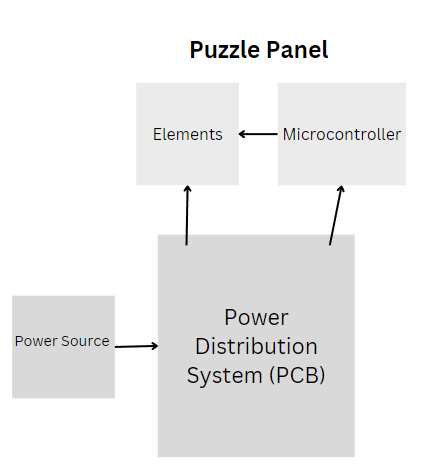
\includegraphics[scale=0.8]{Puzzle Panel tier 1 schematic}
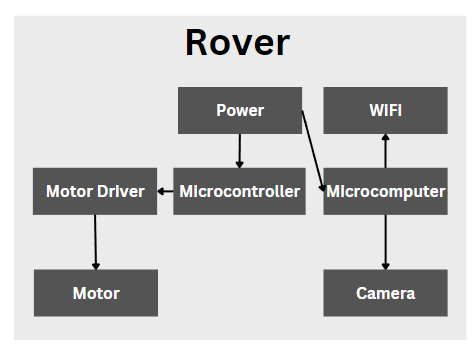
\includegraphics[scale=0.8]{Rover tier 1 schematic}


	Electrical team (EE Capstone):
	
The puzzle panel will be powered by a power source (wall wart) that will connect to a power distribution system (PDS) that will power the actual puzzle panel game. The PDS itself will be able to power each and every hardware with enough power.

	The rover will need a power source that can provide enough power connected to every hardware and also, has a power source that can be efficient and reliable. A power distribution system will be needed to safely distribute enough power to each hardware and also, size of the PDS will be dependent on what the final size of the mechanical system will provide for the PDS to fit in.  

	\subsection{Tier 2 Schematics}
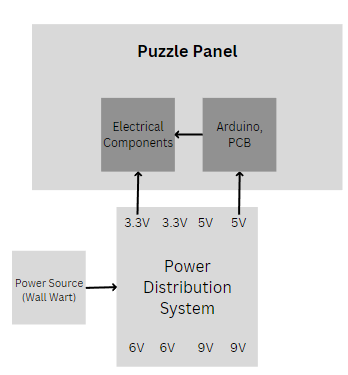
\includegraphics[scale=0.8]{Puzzle panel simplified}
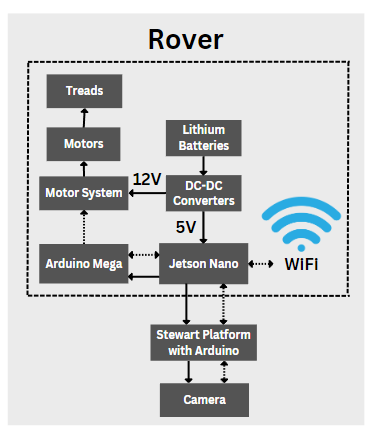
\includegraphics[scale=0.8]{Rover schematic simplified}



	Electrical Team (EE Capstone):
	
The puzzle panel schematic that is shown above details the connection of power for the puzzle panels. The connection starts from the power source which is a wall wart that we will use to power the puzzle panel. The wall wart would output its maximum voltage to the power distribution system (PDS) which then will be distributed to every electrical component. The PDS is constructed to be able to provide different ranges of voltage to meet the power requirements for any electronic component. The puzzle panel itself will be operated by Arduino or PCBs which control the function of the puzzle panel through its connection to the electrical components. Each puzzle panel differs by its own use of electrical components and by the function of its Arduino. 
	
	The simplified Rover Electrical Schematic details the connection from the power source to the rest of the electrical components that are present in the system. The hardware involved are essential for controlling the rover. The Jetson Nano is a microcomputer that runs multiple neuron networks, meaning it can handle multiple tasks at the same time. A Wifi component is built into the Nano which can be controlled wireless without having to control with a physical wire connection. The Arduino Mega is a microcontroller that has the built in code which sends control signals to the motor controllers. The Nano is commanded by the user which the user would send a command to the Nano, and depending on the command which will be sent to the Arduino Mega. This scenario is when both the Nano and the Mega talk to each other with the Nano being controlled by the user have the final say. This relationship works the same way with the Arduino in the stewart platform. The signals that are going to be sent to the motor controllers in the motor system, contain directional/control signals. The motor controllers act like a mini-computer which receives the signals from the Arduino and transmits those signals to the motors which as a result, runs the motors. The arduino with the stewart platform carries the LiDAR camera which monitors live footage and sends back the information in a wireless connection back to the user. The stewart platform is formed with many small stepper motors that reorients the position of the platform from the arduino signals.  

	
Software Team (CE Capstone):

Figure 1 shown above describes the interaction between the Intel RealSense LIDAR L515 with the NVIDIA Xavier. The ROS node that is used as the publisher of the LIDAR image data to then be sent to a subscriber to the image data uses image\_ transport as the library to export the images from the LIDAR to the processing node in a low-bandwidth compressed format to reduce latency. The image processing node has computer vision models within the node to process the image using OpenCV, which is then sent to the Xavier as data that the Xavier will use for further motion logic or displaying the image to the user.

Controller System Design Diagram:

Figure 2 shown above describes the interaction between controllers (Xbox, Playstation, etc type controllers) with the NVIDIA Xavier. There is the package that contains the motion logic that the previously mentioned LIDAR interacts with to send motion controls to the Xavier as well as a ROS node that takes controller inputs and processes them to be sent to the motion logic package. The data going from the controller to the ROS controller is analog data that Linux can already understand and there are pre-existing ROS libraries to use controllers. The controller node itself will send out motion commands to the motion logic package which will then send motion data to the Xavier. We also want to ensure that the controller node itself won't do any illegal inputs so we want to create a connection between the motion logic package and the controller node in case of inputs that were not friendly to the rovers motion.	
	
	\subsection{Tier 3 Schematics}

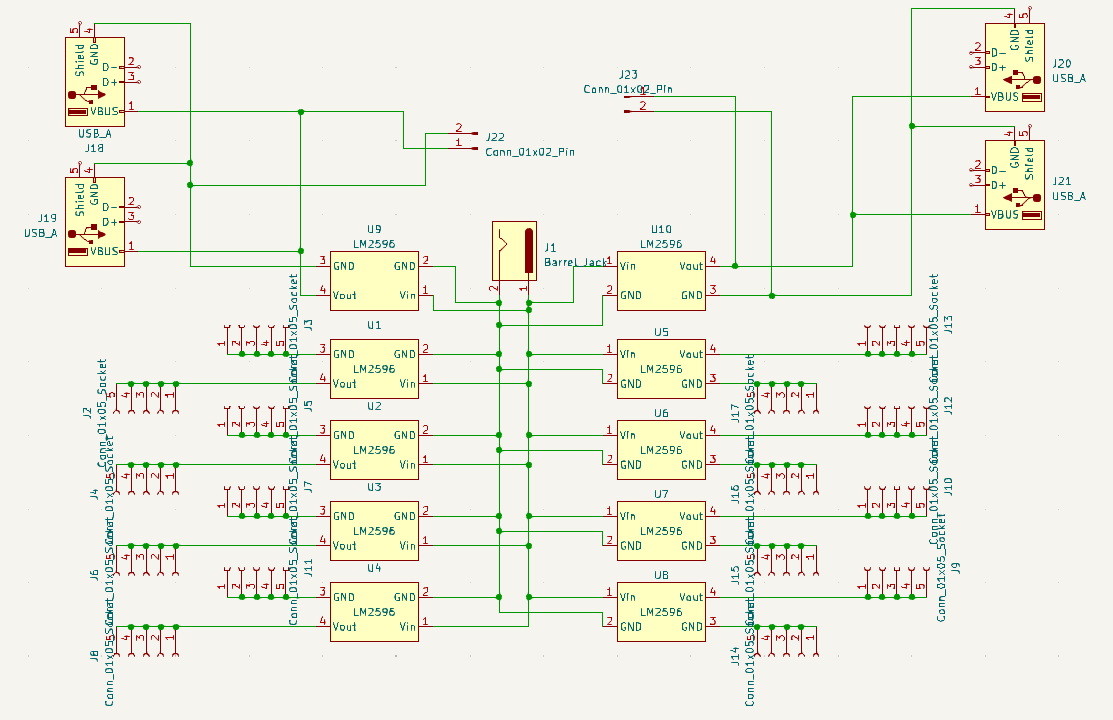
\includegraphics[scale=0.7]{Puzzle Panel schematic 1}	
	
	
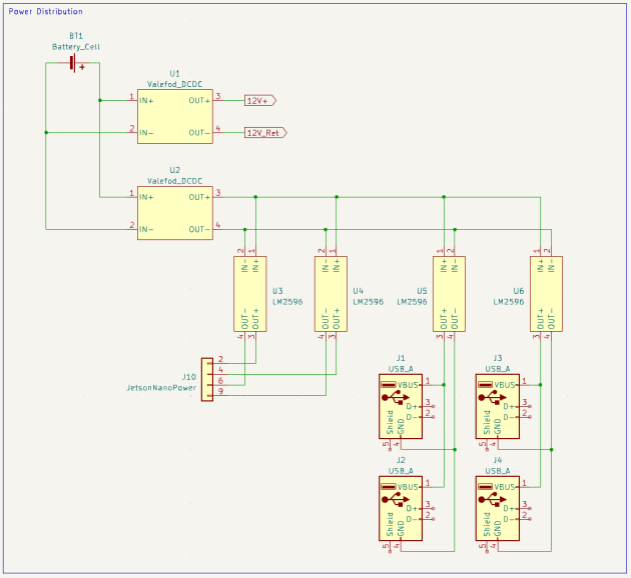
\includegraphics[scale=1.05]{Rover schematic 1}

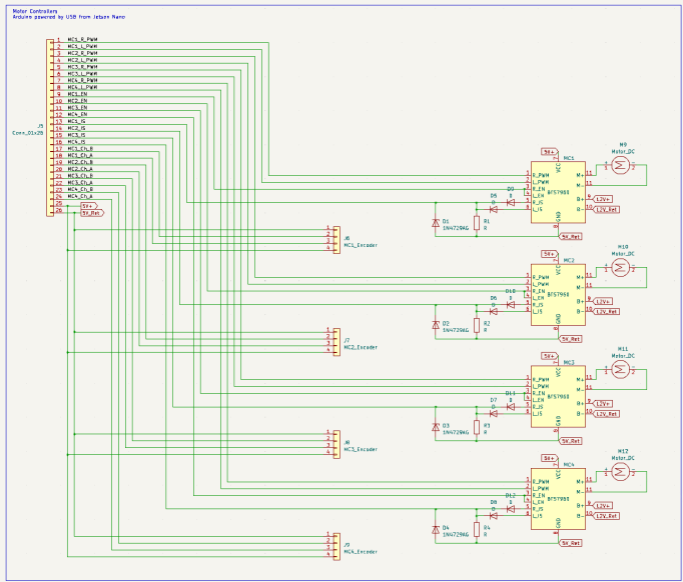
\includegraphics[scale=0.95]{Rover schematic 2}	

		\subsubsection{Electrical Team}
		The PCB of the puzzle panel will start with a wall wart which would output a specified amount of voltage to the PDS. The PDS will be made up of three levels, each level containing rows of buck modules that are placed in parallel and their function is to step-down the input voltage from the wall wart, down to the amount that is needed for an electrical component. Each buck module will distribute different amounts of voltage due to each electrical component within the actual puzzle panel, requiring different levels of voltage.

		The rover will be powered by lithium batteries that can provide enough voltage or power to the whole rover. The 12V DC-DC buck converters which outputs a set amount of voltage of 12V in which the motor controllers are directly powered by. The small buck converters, convert the 12V to 5V which powers the Jetson Nano, Arduino Mega, Stewart platform, and et cetera, which are necessary in the system to control both the distribution of power. 

		The power will be distributed with buck modules to power each component at its needed level. And the step-downed power will then be delivered to the Arduino Mega, Jetson Nano, Motor controllers, and other components which will run the whole rover. This PCB is constructed to use four motor controllers but in this project, two are used to operate the rover. The four USB ports output 5V which are used to provide power to any additional add-ons to the rover, which means different hardware can be added. 
		
		Other miscellaneous elements or components like transistors, diodes, resistors are essential in keeping the digital signals at safe levels, to prevent current/voltage spikes.
		

		\subsubsection{Software/Computer Team}
	
Starting with the LIDAR integration the main connection is between the publisher and subscriber node of the LIDAR image. The publisher node will be outputting a compressed formatted image to the subscriber through the image\_ transport API. Within the processing node (subscriber to the image data) we can use OpenCV to translate the image that is being collected from the publisher to be created into a model that the rover can use to identify what is being shown in the image. This can be done with a point-cloud model and computer vision techniques. After the image is processed, the image itself is sent to the Xavier to display to the user and the image data with motion commands is sent to the motion logic, where the motion logic will then determine whether the images motion data is relevant to motion objectives. The latter is a back and forth process between the subscriber processing node and the motion logic component. 
The second part with Xavier for this capstone project is the controller node. The main connection will be between the controller node that takes in controller information and the motion logic. This will also be a back and forth process between the two since the motion logic may not want to perform the actions that the user is inputting into the controller. 

	\subsection{Estimation of Cost of Goods}
	---Talk about our being a unique capstone and not  needs such a strict cost estimation early on. Nonetheless provide a cost estimate.
	
	We don't have a final estimation of the cost of goods. Major design decisions have to be made by electrical and mechanical leads before a final order can be placed. An early order for the first round of parts has already been placed, see below. 

	\subsection{Schedule}
	We make use of an online, free, Gantt software accessible to anyone. A screenshot of only a portion of our schedule can be seen below. Our project is split into mechanical, electrical, and computer sections, each with 'sub-projects' which have their own schedule prescribed with dates, information, background, etc.

\pagebreak	

\section{Concept Development}

	\subsection{Technology Mapping, Risk Analysis, and Feasibility}
	The minimum product we'll create is a disaster rover, for which we have all the needed components. Functionality will be ensured with the software created to operate well-planned electromechanical systems. Usability will be ensured with effective documentation and simple controls. A well ordered rover with ease of control and robust build will be necessary and capable for further business; though, our client is the UW, so we have little concern for how this would  sell.
	The disaster rover would need to traverse rugged terrain. A compact frame with a well-set center of gravity and tank treads would allow it to path in any environment. Falls or tumbles would be mitigated by a 'domed' upper chassis that ensures it always lands on its base. Operators will be able to connect to it easily and wirelessly, (ideally through browser), and control with easy to understand, video-game based control schemes. All electromechanical systems would interface through robot operating system (ROS) housed on a central, Xavier computer. Focusing on electrical and mechanical systems independently: electronics will convey clean, modular power to various components through LIPO batteries. Clean and modular, I stress again, are the focus; devices like the Xavier have stringent voltage and current regulations. Modularity is desired, as future iterations will see different parts added or subtracted; ideally the only aspects affected here are battery life. Everything is contained on a central PCB, improving physical efficiency further. The mechanical systems need to be robust and sourceable. Through the use of aluminum frame, higher end FDM and resin plastics, and (hopefully) casting, we'll be able to create a protective housing for all electrical and computer components. Motors will be mounted directly to the frame with little (or no) geared transmission, depending on the speed and torque output of what motors exist. A small frame is preferred to minimize stresses. Further research into the mechanical engineering of motion mechanisms is needed before a better description can be provided. 
	The greatest risks are addressed in order: computer, electrical, mechanical. The computer model only addresses the function of interdependent components in extremely ideal conditions. A disaster environment won't be perfect, and the rover needs to get itself out of sticky situations if communication is lost or electromechanical systems aren't behaving perfectly. The electrical system could fail to provide stable enough current or voltage, or locales of high power draw could result in heating that leads to failure. It's possible the arrangement of components doesn't permit a long enough battery, or results in excess inefficiencies. The mechanical systems may fail about shafts or joints, and the production of gears (as they'll be printed) may be outside of tolerance.
	To address the stated risks we need effective testing and redundant systems. Computer models need to simulate circumstances where power delivery or mechanical failure causes issues. Further, boot scripts and backup communication protocols need to exist. Electrical systems have to be tested under every conceivable driven condition, with a focus on clean power. Mechanical systems need to be simulated, constructed with high factors of safety, and modeled physically with test rigs.
 	
 	\subsection{Component Mapping}
 	The electrical system of the rover will consist of many different electrical components that are connected to each other and that can send signal communication to other devices. The system is designed to distribute power to different components from a battery or a single power source. \\
	
The list of hardware components (bound to change after testing and possible redesigns): \\

\textbf{PCB or power distribution system}

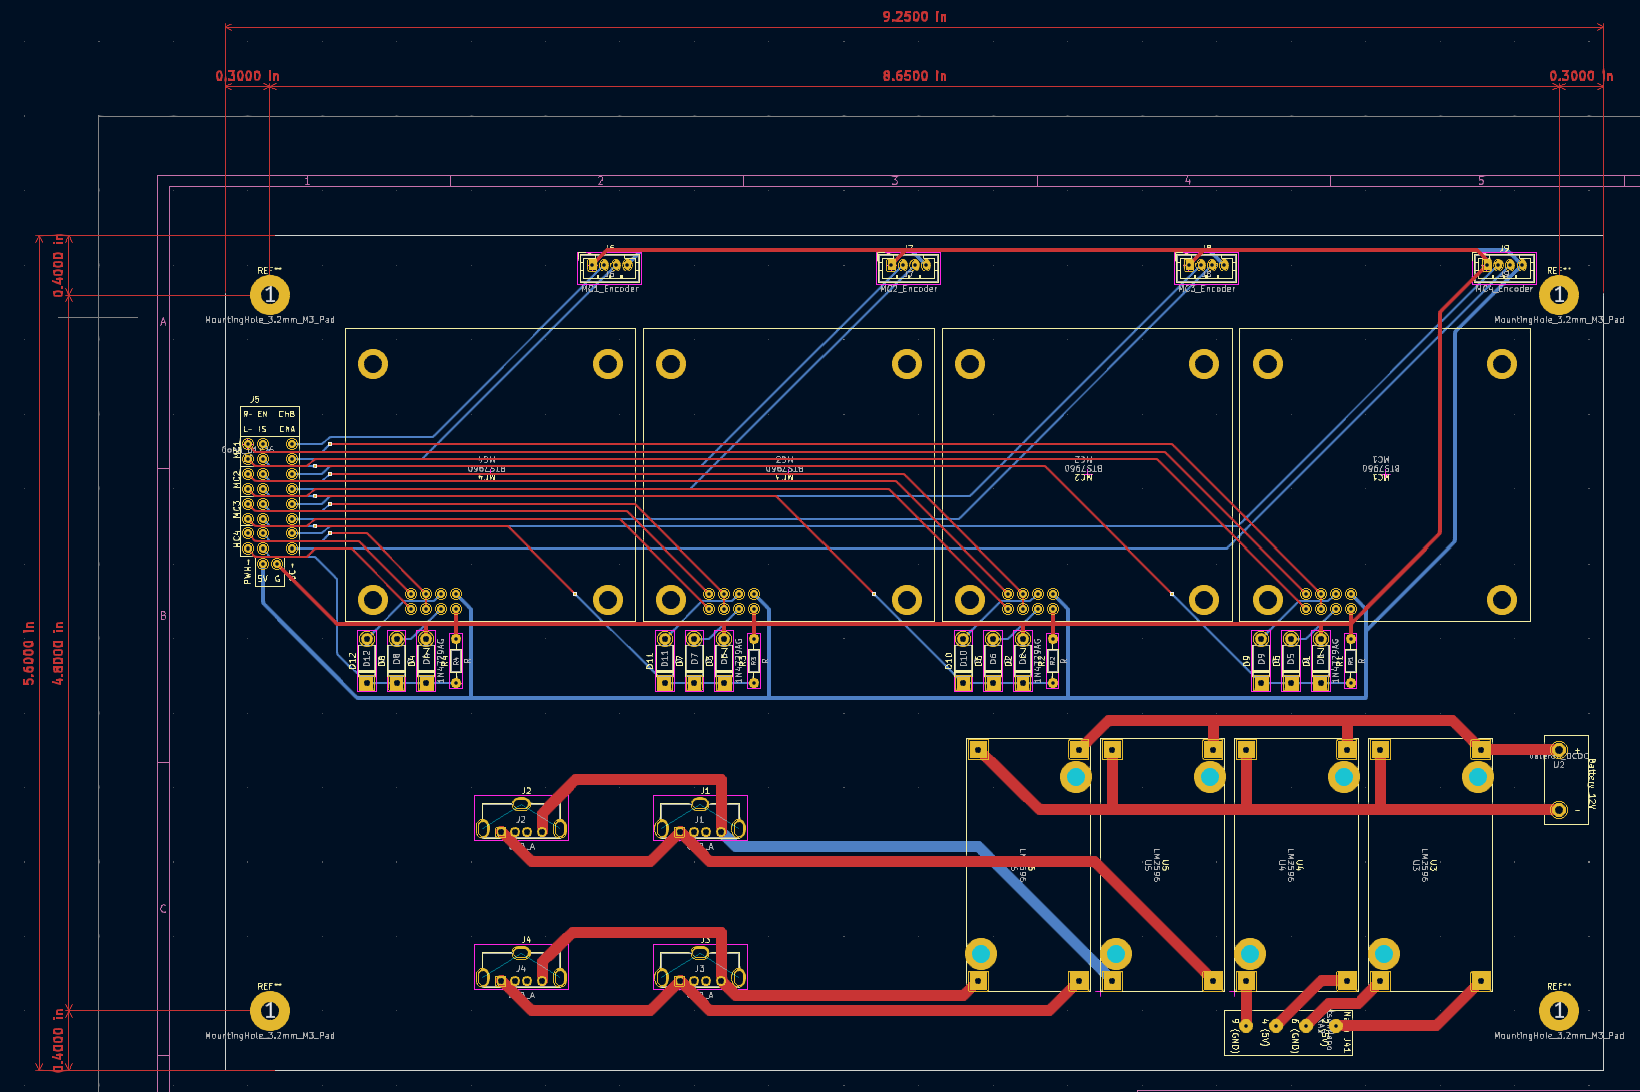
\includegraphics[scale=0.15]{Rover PCB}

\begin{itemize}
\item
	The PCB is designed to distribute power to every electrical hardware from a single power source or battery. And as well as, provide the signal connections for the hardware as they are essential in controlling the functionality of every component.
\end{itemize}


\textbf{Arduino Mega}

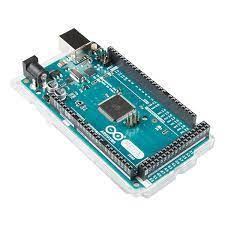
\includegraphics[scale=0.5]{Arduino Mega}

\begin{itemize}
\item
	Arduino Mega is a microcontroller that is designed to control the motors by controlling the motor controllers that control the drivetrain.
\end{itemize}


\textbf{Jetson Nano}

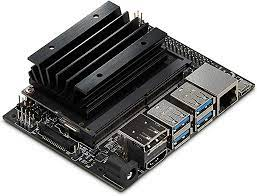
\includegraphics[scale=0.5]{Jetson Nano}

\begin{itemize}
\item
	The Jetson Nano is a small computer that is designed to run multiple neural networks like image processing, object detection, etc. 
\end{itemize}


\textbf{12V DC-DC Buck Converters}

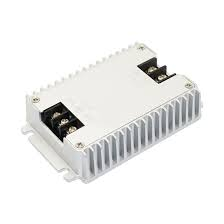
\includegraphics[scale=0.5]{12V DC-DC buck converter}

\begin{itemize}
\item
	The 12V DC-DC buck converter is used to step down any voltage larger than 12V down to its assigned level of 12V.
\end{itemize}


\textbf{LM2596 Buck Converters}

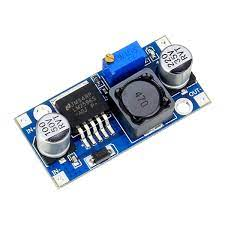
\includegraphics[scale=0.5]{LM2596 bucks}

\begin{itemize}
\item
	The LM2596 buck converters are designed to step down or drop down the voltage that is needed by the electrical components to be able to functionally run. And it's adjusted by a potentiometer that controls the voltage level output.
\end{itemize}


\textbf{LiDAR camera}

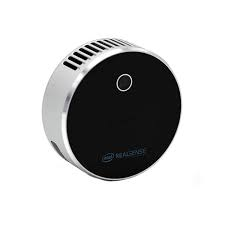
\includegraphics[scale=0.5]{LiDAR Camera}

\begin{itemize}
\item
	The LiDAR camera is tasked to provide image mapping to the rover.
\end{itemize}


\textbf{BTS7960 Motor Controller}

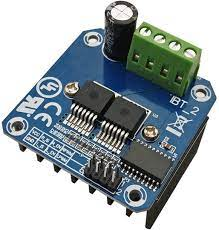
\includegraphics[scale=0.5]{BTS7960 Motor Driver}

\begin{itemize}
\item
	The motor controller is used to receive signals from the Arduino Mega and delivers it to the actual motors of the drivetrain.
\end{itemize}

\textbf{12V Planetary Gear Motors}

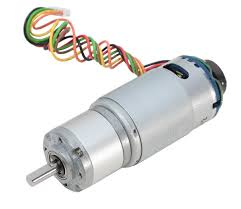
\includegraphics[scale=0.5]{Gear motor 12V planetary}

\begin{itemize}
\item
	The 12V planetary motors are used to drive the whole rover which are controlled by the BTS7960 motor controller through digital signals from the Arduino Mega.
\end{itemize}

\underline{Risk identification}

\begin{itemize}
\item
	One of the major risks or dangers for the electrical system is the probability of overheating which will cause a fire hazard. This will cause permanent damage to many of the components on the rover. The battery and the components that needed the most power are at risk of this danger, so sufficient protection for these parts will lower the risk of this danger.

\item
	The risk of the motors running too much or insufficient torque will cause different amounts of currents to be drawn from the battery. This current spike will cause damage to the electrical hardware that is directly connected to the battery and cause a fire hazard. The mechanical components will also face damage as a result.
\end{itemize}

\underline{Software System}

The software system of the rover will be centered around using the Robotic Operating System - ROS, which is an open source robotics middleware. The system is designed to live on the NVIDIA Xavier and Raspberry PI on the rover and consists of multiple sections of code that interact within the ROS environment. The software system is used to provide command and control for the rover. The Raspberry PI and NVIDIA Xavier pictures can be seen in Figure D1 and Figure D2 respectively. \\

List of ROS packages (bound to change after testing and possible redesigns): \\

\textbf{LIDAR Package}
\begin{itemize}
\item
	This package consists of a publisher node for the LIDAR image data and two subscriber nodes for outputting the image data as either an imaging processing node or an image viewing node. The image processing node is able to process the image and send corresponding motion data to the main motion logic package. The image viewing node is used to display the image that is coming out of the publisher node to wherever the output is required live.
\end{itemize}

\textbf{Controller Package}

\begin{itemize}
\item
	This package consists of a publisher node for the controller data and currently one subscriber node that processes the controller data to be sent to the main motion logic package. 
\end{itemize}

\textbf{Motion Logic Package}

\begin{itemize}
\item
	This package consists of a publisher node that takes motion data from the LIDAR or controller to determine the motion of the rover. The subscriber will be a middle node that connects to the Raspberry PI which is used as the motor controller for the motors on the rover. 
\end{itemize}

\underline{Risk Identification}

\begin{itemize}
\item
	A major risk is the LIDAR node creating a false LIDAR map of the surrounding area and thus sending false information to the motion logic package. We can mitigate this by adding in additional logic to prioritize using controller motion data compared to the LIDAR mapping data. 

\item
	Another risk is the motion logic not having enough logic within it to ensure that the rover does not make false moves that may endanger the rover itself. This risk can be mitigated through edge case testing and ensuring the motion logic corresponds correctly with rover movements. 

\item
	The rover system depends on a fully functional user interface for all interactions. If one of the user interface functions does not work correctly, the specific functionality will be affected and not be easily accessed by the user through the application. 
\end{itemize}
	\subsection{Design Strategy, Concept Development, and Concept Risk Identification \& Mitigation}


		\subsubsection{Technology Mapping, Component Technology Research}
		
		The Project GANTT chart can be added here for the technology mapping image.

		\subsubsection{Electrical}
		The electrical circuit or model will be tested with the mechanical models, and the approximate date of testing will take place from the end of April to May. Testing will involve making sure connections are stable and all electrical components are functioning correctly and correspondingly communicate with each other. 
		
Future testing of electrical components and their functions:
\begin{itemize}
\item
The connections between components

\item
PCB functionality

\item
Jetson Nano connection

\item
Arduino Mega and Drivetrain connection

\item
Battery and power/current performance
\end{itemize}

The main risk of the electrical circuit or model is that the electrical connection between any electrical components has failed. The risk mitigation can involve:

\begin{itemize}
\item
Rewiring/replacing wires, checking every connection between every electrical component.

\item
Replacing old/faulty components with new ones can decrease the risk of circuit failure.
\end{itemize}

Another risk of the electrical circuit is the uneven distribution of power to any electrical component through voltage/current spikes and voltage/current noise. The risk mitigation can involve:

\begin{itemize}
\item
Adding new electrical components that are used to mitigate or decrease voltage/current spikes.

	\begin{itemize}
		\item
		Snubber diodes, bypass capacitors, transistors, and any other component that can prevent undesirable effects. 
	\end{itemize}
	
\item
Adding fuses can be used as a fail-safe to prevent the failure of the entire electrical system.
\end{itemize}


Another risk is any wire disconnecting during a test run which can cause an open circuit with the current not flowing in the intended direction and flowing towards volatile electrical components. The risk mitigation can involve:

\begin{itemize}
\item
Adding new electrical components that are used to block current.

	\begin{itemize}
		\item
		Blocking diodes and transistors can protect volatile components by preventing or blocking current from flowing backwards to a vulnerable component. 
	\end{itemize}
\end{itemize}

Future risks will be identified with further testing of the models.

		\subsubsection{Mechanical}
		\subsubsection{Firmware and Software}
		The rover system will be tested within computer simulation and with the rover itself. The testing will take place between April to May and will test the components that were created such as the LIDAR, controller, and motion logic packages. We will also test that the interaction between all the packages are working as expected. 
		
\begin{itemize}
\item
	LIDAR system testing will consist of ensuring that the image display is displayed correctly on the outputting display and that the image processing node is providing motion logic data that is accurate to the map that the LIDAR creates.
	
\item
	Controller system testing will consist of input testing of single or multiple input prompts and ensuring that the rover can respond to the motion logic that comes out of the controller system. 
	
\item
	Motion logic system testing will coincide with controller system testing as we need inputs to ensure that the motion logic is moving the right motors and the connection between the Xavier and PI are correct. In this we will validate that the motion logic system can turn the correct motor on command and can work independently from the LIDAR or controller if we do manual inputs through the console. To reduce the risk about the incorrect movements from the controller to the motion logic, we will run edge cases with a multitude of inputs to the controller and observe how the motion logic responds to them.
\end{itemize}

		\subsubsection{Human Interaction Models}
		The main interaction between the user and the prototype will be through a PC and possibly an Xbox controller which would control the rover. The PC will allow the user to start the rover through the ROS language and be able to test the prototype. The Xbox controller would be used to navigate the rover with joint sticks to do basic operations. And this controller works best for the user to control the rover and wouldn't require them to know ROS. The risk mitigation involves allowing the user to use the software without first-hand knowledge and being able to test the prototype with ease. This would also allow easy control and having it be user-friendly.

		\subsubsection{System Interface Modeling, Testing, and Risk Analysis}
Testing the system interface of the rover, we would ensure that the connections between the interface are functioning accurately. Some of the components which we would be testing are the connection for the LiDAR camera. 

The main risk of the system interface would be the failure in the connection between the devices. Mitigating the risk would involve:

\begin{itemize}
\item
Testing each connection between systems and their interface functionality.

\item
Testing the LiDAR camera to ensure that the mapping is accurate and readable. 
\end{itemize}

The testing of these systems will be finished around May and more progress will be done as the team continues to design and build the actual systems.

\section{Methodology}

What data you will need to collect, and how. 
What are the industry standards used in this project? 

Electrical:

The data that we need to collect involves current/power performance when the entire rover operates. And also, the duration the batteries can last under a full operation by measuring the rate of the current. A special tool called a Clamp Meter is used to measure current values in real time. And it also, doesn't require wire to wire connection to measure as Clamp Meter measures through the magnetic fields from where the current is present. Acquiring the current measurements help determines the overall performance of the rover, its battery life and overall efficiency.

The industry standards used, is the usage of a professional PCB design program KiCad EDA which famous companies known for inventing Electrical Engineering projects like Adafruit which is known to design arduinos which are used in this project, Digi-Key Electronics which is known to manufacture standardized and basic electrical components, most are utilized to create the power distribution PCB of the rover.

\section{Results and Discussion}

Electrical:

The testing for the results in measuring the current/power performance of the rover are successful. We monitored the current levels going into the motor controllers running at 12V during a simple operational maneuver and the rover used around 1.5A when operating on flat ground. The next test involve operating the rover on dirt ground and driving over uneven terrain. Introducing dirt and uneven terrain would require the rover to draw more current since dirt and uneven terrain cause friction and resistant force for the rover to overcome. The results of the tests are successful with the rover operating over dirt in 1.6A to 1.7A and for uneven terrain, around 2.0A was used. The next major test involve moving the rover against the wall, to test the rover when it meets a maximum physical force. The overall current level reached to 3.3A which is more than twice the amount the rover used normally. These values help determine how long the rover perform under each of these environmental conditions. Additionally, there were no electrical hardware failures through each test, which we can conclude that the entire circuit is protected from voltage/current spikes or wire disconnects. And the current used in these conditions, are less than expected so we can safely assume the rover can handle harsher terrain and conditions.

Monitoring the power efficiency and delivery of the Puzzle Panel PCB was successful. Every buck module are able to output the specified voltage based on the adjustment of their potentiometers. And when powering the hardware and the puzzle panel elements, there were no signs of electrical failures. The most number of elements that are connected to the PCB are three and when they operate, they draw 0.7A to 1A. With other slots of power and USBs in the PCB that are available, additional hardware or puzzle elements can be powered from the PCB. And with the performance of power not showing signs of failure, we can safely assume the Puzzle Panel PCB can handle powering multiple hardware and components at once.

\section{Summary, Conclusion and Future Perspectives}
Summary section (in bullet form)
key open actions and concerns
Future perspectives 

Electrical:

\begin{itemize}
\item
Rover PCB: Redesign the layout of the components to manage space for better wire to wire connections, selecting newer and improved components that are more efficient and easy to use. Also, replacing any faulty or old hardware to prevent fatal electrical failures or accidents. 

\item
Puzzle Panel PCB: Redesign the layout of the board to provide many more different alternatives to power different range of hardware, and select newer components to improve maximum power efficiency.

\end{itemize}

\section{Acknowledgments}

\section{Bibliography} 

\section{Appendices and Supplement Data}  

\section{User Manual}

Electrical User Manual:

Puzzle Panel - 1. 

Rover - 

\end{document}
